\chapter{Introduzione alla programmazione lineare a numeri interi}

Si consideri il seguente problema.
\begin{flalign*}
	& Min\ cx \\
	& \ \ \ \ \ \ \ Ax=b \\
	& \ \ \ \ \ \ \ x\ge 0 \\
	& \ \ \ \ \ \ \ x\ intero
\end{flalign*}
Le variabili devono assumere valori interi:
\begin{flalign*}
	& Es:\ \ x_{i}=Numero\ di\ uomini\ che\ devono\ essere\ assegnati\ al\ lavoro\ i. \\
	& \ \ \ \ \ \ \ \ \ \ \ =\ Numero\ di\ automezzi\ che\ devono\ operare\ il\ trasporto\ lungo\ la\ "tratta\  i" \\
	& \ \ \ \ \ \ \ \ \ \ \ =\ Numero\ di\ macchine\ da\ utilizzare\ nella\ lavorazione\ i
\end{flalign*}

\section{Arrotondamento ad una soluzione non-intera}
Si risolva il problema ignorando i vincoli [$x: intero$].
Le variabili che risultano non intere, nella soluzione ottima del problema continuo, vengano arrotondate al valore intero pi\`u vicino.
\begin{flalign*}
	& Es:\ \ Min\ z=-2x_{1}+3x_{2} \\
	& \ \ \ \ \ \ \ \ \ \ \ \ \ \ \ \ \ \ \ \ \ \ \ \ x_{1}+x_{2}\ge 3 \\
	& \ \ \ \ \ \ \ \ \ \ \ \ \ \ \ \ \ \ \ \ \ \ \ \ 3x_{1}+x_{2}\le 6 \\
	& \ \ \ \ \ \ \ \ \ \ \ \ \ \ \ \ \ \ \ \ \ \ \ \ x_{2}\le 5 \\
	& \ \ \ \ \ \ \ \ \ \ \ \ \ \ \ \ \ \ \ \ \ \ \ \ x_{1},\ x_{2}\ge 0\ ed\ intere
\end{flalign*}
\begin{figure}[h]
	\centering
	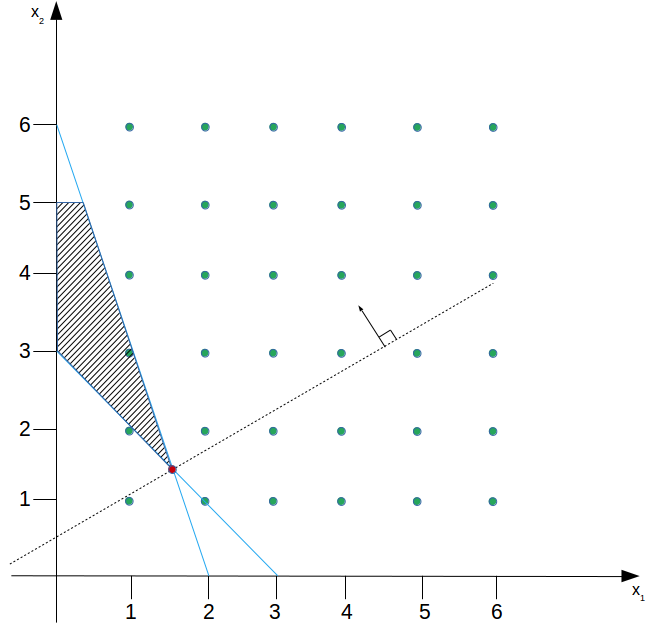
\includegraphics[height=12cm]{images/graph6.png}
	\label{fig:SoluzioneOttimaContinua1}
	\caption[]{\\Soluzione continua: $z=\frac{3}{4}$; $x_{1}=\frac{3}{2}$, $x_{2}=\frac{3}{2}$ \\ Soluzione intera: $z=4$; $x_{1}=1$, $x_{2}=2$}
\end{figure}

In questo esempio la soluzione arrotondata coincide con la soluzione ottima.

\begin{flalign*}
& Es:\ \ Min\ z=8x_{1}+6x_{2} \\
& \ \ \ \ \ \ \ \ \ \ 4x_{1}+3x_{2}\ge 6 \\
& \ \ \ \ \ \ \ \ \ \ x_{1},\ x_{2}\ge 0\ ed\ intere
\end{flalign*}
\begin{figure}[h]
	\centering
	\captionsetup{justification=centering}
	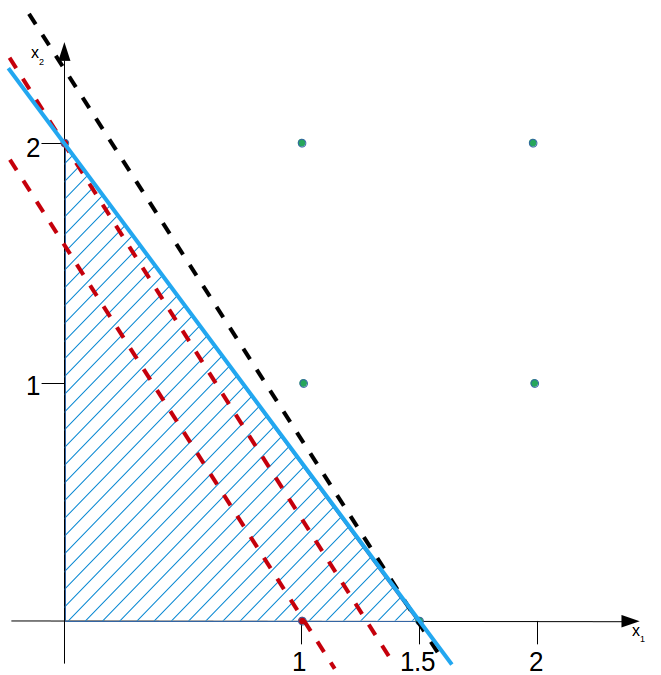
\includegraphics[height=13cm]{images/graph7.png}
	\label{fig:SoluzioneOttimaContinua2}
	\caption[]{\\ Soluzione continua: $z=12$; $x_{1}=1,5$, $x_{2}=0$ \\ Soluzione arrotondata $z=8$; $x_{1}=1$, $x_{2}=0$ \\ Soluzione intera: $z=10$; $x_{1}=0$, $x_{2}=2$}
\end{figure}

La soluzione arrotondata si discosta notevolmente dalla soluzione ottima.

\begin{flalign*}
& Es:\ \ Min\ z=8x_{1}+6x_{2} \\
& \ \ \ \ \ \ \ \ \ \ 4x_{1}+3x_{2}\ge 6 \\
& \ \ \ \ \ \ \ \ \ \ x_{1},\ x_{2}\ge 0\ ed\ intere
\end{flalign*}
\begin{figure}[h]
	\centering
	\captionsetup{justification=centering}
	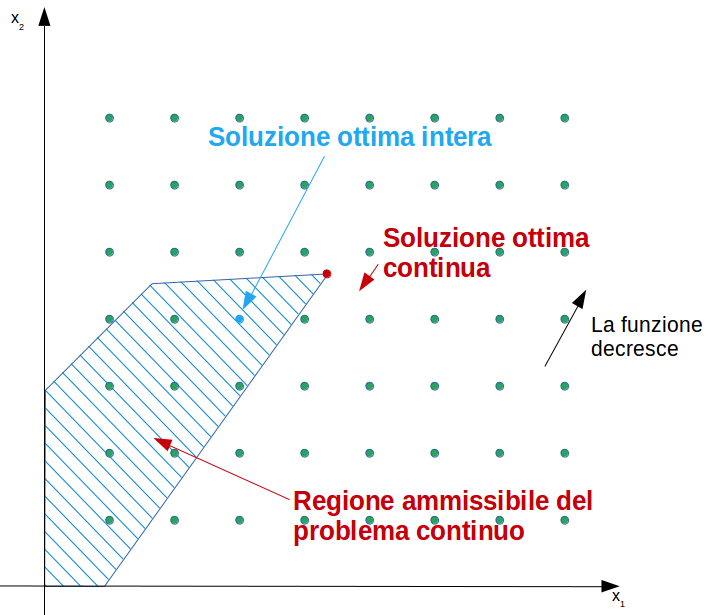
\includegraphics[height=14cm]{images/graph8.png}
	\label{fig:SoluzioneOttimaContinua3}
\end{figure}

I quattro punti interi pi\`u vicini alla soluzione continua non sono ammissibili.
\newpage

\section{Unimodularit\`a}
La matrice intera A di $m$ righe ed $n$ colonne \`e totalmente unimodulare se ogni sua sottomatrice quadrata B non singolare \`e unimodulare, ovvero $det(B)=\pm 1$.\\

\textbf{Teorema.}

Se la matrice intera $A$ \`e totalmente unimodulare allora tutti i punti estremi dell'insieme pd. convesso $X={x:\ Ax=b,\ x\ge 0}$ sono interi per ogni vettore intero $b$.\\

\textbf{Dimostrazione.}

Sia B una base ammissibile e $x_{b}$ le variabili base: $Bx_{B}=b$.\\
Per la regola di Cramer:
\begin{flalign*}
	& x_{b_{i}}=\frac{\det(B_{i})}{\det(B)}
\end{flalign*}
Dove $B_{i}$ si ottiene da $B$ sostituendo la i-esima colonna di $B$ con $b$. \`E ovvio che $\det(B_{i})$ \`e un numero intero e quindi anche ciascun $x_{B_{i}}$ \`e intero.\\

\textbf{Teorema.}

Una matrice intera $A$ i cui elementi sono $0, +1, -1$ \`e totalmente unimodulare se:
\begin{enumerate}
	\item In ogni colonna $A$ compaiono al pi\`u due elementi non-nulli (cioè $1,-1$);
	\item L'insieme delle righe R pu\`o essere suddiviso in due insieme disgiunti $R_{1}$ e $R_{2}$ ($R_{1}\cup R_{2}=R$) per cui:
	\begin{enumerate}
		\item Se una colonna contiene due elementi non-nulli dello stesso segno allora la riga corrispondente ad uno dei due elementi appartiene a $R_{1}$ mentre la riga relativa all'altro elemento \`e in $R_{2}$;
		\item Se una colonna contiene due elementi di segno opposto entrambe le righe appartengono allo stesso insieme.
	\end{enumerate}
\end{enumerate}

\textbf{Esempi.}

\begin{tabular}{cc}
	$ A=\begin{bmatrix}
		-1 & 1 & 1 & 0 & 0 & 0 \\
		0 & 0 & -1 & -1 & 1 & 1 \\
		0 & 0 & 0 & 0 & 0 & -1 \\
		1 & -1 & 0 & 1 & -1 & 0 \\
	\end{bmatrix},$ &
	$A = \begin{bmatrix}
		1 & 1 & 1 & 0 & 0 & 0 & 0 & 0 \\
		0 & 0 & 0 & 1 & 1 & 1 & 0 & 0 \\
		0 & 0 & 0 & 0 & 0 & 0 & 1 & 1 \\
		1 & 0 & 0 & 1 & 0 & 0 & 1 & 0 \\
		0 & 1 & 0 & 0 & 1 & 0 & 0 & 1
	\end{bmatrix}$ \\
	\begin{minipage}{0pt}
		\vskip 10pt
		\begin{itemize}
			\item[$R={1,2,3,4}$]
			\item[$R_{1}={1,2,3,4}$]
			\vspace{-6mm}
			\item[$R_{2}=\emptyset$]
			\vspace{-6mm}
		\end{itemize}
	\end{minipage} &
	\begin{minipage}{0pt}
		\vskip 10pt
		\begin{itemize}
			\item[$R={1,2,3,4,5}$]
			\item[$R_{1}={1,2,3}$]
			\vspace{-6mm}
			\item[$R_{2}={4,5}$]
			\vspace{-6mm}
		\end{itemize}
	\end{minipage} \\
\end{tabular}

La totale unimodularit\`a della matrice $A$ \`e \textbf{condizione sufficiente} affinch\`e la soluzione ottima $x^{*}$ sia intera per
\begin{flalign*}
	& Min\ cx\\
	& \ \ \ \ \ \ \ Ax=b\ (b\ intero)\\
	& \ \ \ \ \ \ \ x\ge 0
\end{flalign*}
La condizione non \`e \textbf{necessaria}.\\\\
\textbf{Esempio:}

dato il sistema di vincoli
\begin{flalign*}
	& 6x_{1}+x_{2}=7 \\
	& 2x_{1}+x_{2}=3
\end{flalign*}
L'unica soluzione \`e ($x_{1}=1,\ x_{2}=1$) mentre la matrice
\begin{center}
	$ A=\begin{bmatrix}
	6 & 1 \\
	2 & 1
	\end{bmatrix}$	
\end{center}
non risulta essere totalmente unimodulare.
\newpage

\section{Metodo dei piani di taglio}
Sia dato il problema
\begin{displaymath}
ILP
	\begin{cases}
	\ Min\ z_{ILP}=cx\\
	\ \ \ \ \ \ \ \ \ \ \ \ \ \ \ \ \ \ A x = b\\
	\ \ \ \ \ \ \ \ \ \ \ \ \ \ \ \ \ \ x \ge 0\ e\:intero
	\end{cases}
\end{displaymath}
Supponiamo $A$,$c$,$b$ interi.\\
Si consideri il problema rilassato che si ottiene da $ILP$ ignorando i vincoli di interezza.\\
Indichiamo tale problema con \textbf{\emph{LP}}.
\begin{displaymath}
	LP
	\begin{cases}
	\ z_{LP}\ =\ Min\ cx\\
	\ \ \ \ \ \ \ \ \ \ \ \ \ \ \ \ \ \ \ ax=b\\
	\ \ \ \ \ \ \ \ \ \ \ \ \ \ \ \ \ \ \ x\ge 0\\
	\end{cases}
\end{displaymath}
È noto che $z_{LP}\le z_{ILP}$.

\subsection{Piani di taglio}
Si risolva $LP$; se la soluzione è intera tale soluzione è anche l'ottimo di $ILP$.

Altrimenti vengono aggiunti a $LP$ vincoli, \emph{che non escludono soluzioni intere}, fino a che la soluzione del problema $LP$ risultante non risulti intera.

\begin{figure}[!htb]
	\minipage{0.32\textwidth}
	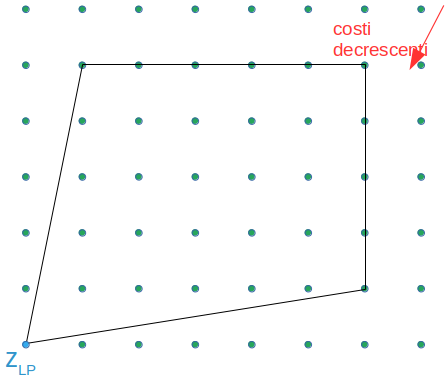
\includegraphics[width=\linewidth]{images/graph9.png} 
	(A)
	\label{fig:pianiditaglio1}
	\endminipage\hfill
	\minipage{0.32\textwidth}
	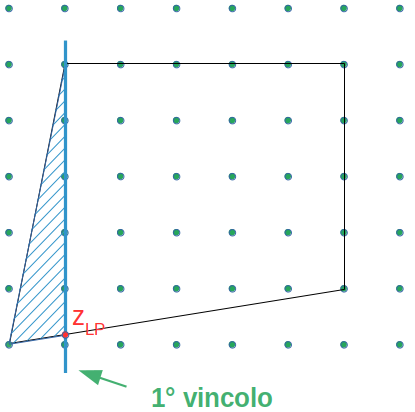
\includegraphics[width=\linewidth]{images/graph10.png}
	(B)
	\label{fig:pianiditaglio2}
	\endminipage\hfill
	\minipage{0.32\textwidth}%
	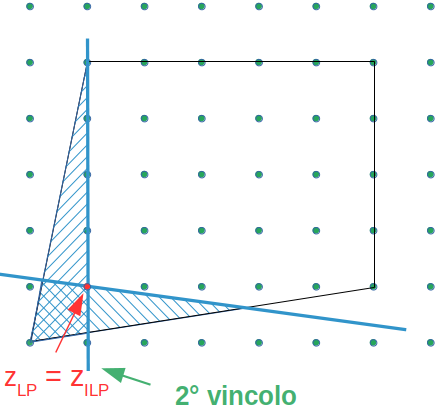
\includegraphics[width=\linewidth]{images/graph11.png}
	(C)
	\label{fig:paniditaglio3}
	\endminipage
\end{figure}

In $(A)$ viene mostrata la regione ammissibile di $LP$ ed il punto di ottimo.

In $(B)$ viene mostrata la regione ammissibile di $LP$ più un vincolo che rende non-ammissibile l'ottimo ottenuto in $(A)$ ma che non esclude nessuno dei punti interi.

In $(C)$ viene mostrato come l'aggiunta di un secondo vincolo rende la soluzione intera.\\
\textbf{Nell'esempio sono sufficienti 2 vincoli per rendere la soluzione intera.}
In generale bisogna aggiungere vincoli fino a che la soluzione non risulti intera o si scopra che il problema non ha soluzioni intere.

\subsection{Gomory cuts}
Si consideri il tableau ottimo relativo a LP:

\begin{table}[h]
	\centering
	\begin{tabular}{llllllcccccccc}
		&                       z & $x_{1}$ &    & \dots &     &      & $x_{m}$ & $x_{m+1}$     & \dots & $x_{j}$     & \dots & $x_{n}$     & \\ \cline{2-14}
		& \multicolumn{1}{|l|}{1} & 0       &    & \dots &     &      & 0       &               &     &             &     &             & \multicolumn{1}{|l|}{} \\ \cline{2-14}
		$x_{1}$ & \multicolumn{1}{|l|}{}  & 1       &    &     &     &      &         &               &     &             &     &	           & \multicolumn{1}{|l|}{$\bar{b}_{1}$} \\
		& \multicolumn{1}{|l|}{}  &         & 1  &     &     &      &         &               &     &             &     &             & \multicolumn{1}{|l|}{} \\
		& \multicolumn{1}{|l|}{}  &         &    & \dots &     &      &         &               &     &             &     &             & \multicolumn{1}{|l|}{} \\
		$x_{r}$ & \multicolumn{1}{|l|}{}  &         &    &     & 1   &      &         & $y_{r}^{m+1}$ & \dots & $y_{r}^{j}$ & \dots & $y_{r}^{n}$ & \multicolumn{1}{|l|}{$\bar{b}_{r}$} \\
		& \multicolumn{1}{|l|}{}  &         &    &     &     & \dots  &         &               &     &             &     &             & \multicolumn{1}{|l|}{} \\
		$x_{m}$ & \multicolumn{1}{|l|}{}  &         &    &     &     &      & 1       &               &     &             &     &             & \multicolumn{1}{|l|}{$\bar{b}_{m}$} \\ \cline{2-14}
	\end{tabular}
\end{table}

Supponiamo che la soluzione ottima sia non intera.\\
Sia $\bar{b}_{r}$ non intero.

L'equazione associata a $x_{r}$ è:
\begin{equation}\label{eq:2.1}
x_{r} + \sum_{j=m+1}^{n} y_{r}^{j} x_{j} = \bar{b}_{r}
\end{equation}
Poniamo:
\begin{equation*}
y_{r}^{j} = I_{r}^{j} + F_{r}^{j}\text{, dove }I_{r}^{j} = \lfloor y_{r}^{j} \rfloor,\ (0 \le F_{r}^{j} < 1)
\end{equation*}

Inoltre:
\begin{equation*}
\bar{b}_{r} = I_{r} + F_{r} \text{ essendo } 0 \le F_{r} < 1
\end{equation*}

Sostituendo, la \ref{eq:2.1} diviene:
\begin{equation*}
x_{r} + \sum_{j=m+1}^{n} (I_{r}^{j} + F_{r}^{j}) x_{j} = (I_{r} + F_{r})
\end{equation*}
o anche:
\begin{equation*}
\underbrace{x_{r}+\sum_{j=m+1}^{n} I_{r}^{j} x_{j} - I_{r}}_\text{intero per ogni $x$ intero} = \underbrace{F_{r} - \sum_{j=m+1}^{n} F_{r}^{j}x_{j}}_\text{< 1 per $x\ge0$}
\end{equation*}
Ne segue:
\begin{equation*}
F_{r} - \sum_{j=m+1}^{n} F_{r}^{j} x_{j} \le 0
\end{equation*}
La soluzione corrente non soddisfa il vincolo \ref{eq:2.1} in quanto $x_{j} = 0$, $j=m+1,\dots,n$ mentre $F_{r}>0$ poiché $\bar{b}_{r}$ si è supposto non intero.\\
Se il vincolo \ref{eq:2.1} viene aggiunto al problema $LP$ allora la soluzione corrente risulterà non ammissibile.\\
Per determinare una nuova soluzione che soddisfi il vincolo \ref{eq:2.1} può essere impiegato il \emph{Simplesso Duale} partendo dal tableau ottimo relativo alla soluzione corrente.\\
Al tableau va aggiunto il vincolo:
\begin{equation*}
- \sum_{j=m+1}^{j} F_{r}^{j} x_{j} + s = -F_{r}
\end{equation*}
La nuova variabile slack $s$ è una nuova variabile base.\\
Il nuovo tableau è non ammissibile per il Primale ma duale ammissibile.\\

\textbf{Esempio.}
\begin{flalign*}
	& Min\,\;- x_{2} \\
	& \ \ \ \ \ \ \ \ \ \ 3x_{1}+2x_{2}\le 6 \\
	& \ \ \ \ \ \ \,-3x_{1}+2x_{2}\le 0 \\
	& \ \ \ \ \ \ \ \ \ \ \ \,x_{1},\ x_{2}\ge 0 \\
	& \ \ \ \ \ \ \ \ \ \ \ \,x_{1},\ x_{2}\ intere\\
\end{flalign*}
Si noti che l'ottimo cade nel punto $x=(1;1)$.

\centerline{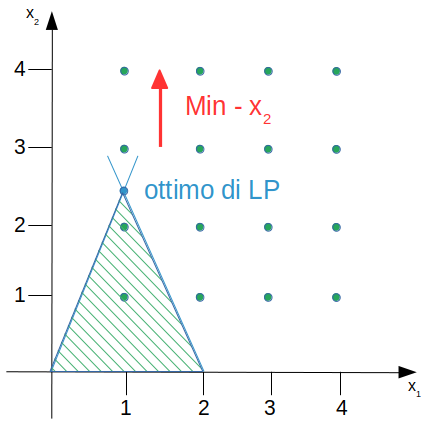
\includegraphics[height=9cm]{images/graph12.png}}

\begin{table}[h]
	\centering
	\begin{tabular}{ccccccc}
				&                       z & $x_{1}$ & $x_{2}$  & $x_{3}$ & $x_{4}$ &  RHS  \\ \cline{2-7}
			z	& \multicolumn{1}{|l|}{1} & 0       & 1        & 0       & 0       & \multicolumn{1}{|l|}{0} \\ \cline{2-7}
		$x_{3}$ & \multicolumn{1}{|l|}{0} & 3       & 2        & 1       & 0	   & \multicolumn{1}{|l|}{6} \\
		$x_{4}$ & \multicolumn{1}{|l|}{0} & -3      & {\LARGE \textcircled{\normalsize $2$}}        & 0       & 1       & \multicolumn{1}{|l|}{0} \\ \cline{2-7}
	\end{tabular}
\end{table}

\begin{table}[!h]
	\centering
	\begin{tabular}{lllllll}
		        &                       z & $x_{1}$ & $x_{2}$  & $x_{3}$ & $x_{4}$ &  RHS  \\ \cline{2-7}
		      z & \multicolumn{1}{|l|}{1} & 3/2     & 0        & 0       & -1/2    & \multicolumn{1}{|l|}{0} \\ \cline{2-7}
		$x_{3}$ & \multicolumn{1}{|l|}{0} & {\LARGE \textcircled{\normalsize $6$}}   & 0       & 1 & -1  & \multicolumn{1}{|l|}{6} \\
		$x_{2}$ & \multicolumn{1}{|l|}{0} & -3/2    & 1        & 0       & 1/2     & \multicolumn{1}{|l|}{0} \\ \cline{2-7}
	\end{tabular}
\end{table}

\begin{table}[!h]
	\centering
	\begin{tabular}{lllllll}
				&                         & $x_{1}$ & $x_{2}$  & $x_{3}$ & $x_{4}$ &  RHS  \\ \cline{2-7}
			z	& \multicolumn{1}{|l|}{1} & 0       & 0        & -1/4    & -1/4    & \multicolumn{1}{|l|}{-3/2} \\ \cline{2-7}
		$x_{1}$ & \multicolumn{1}{|l|}{0} & 1       & 0        & 1/6     & -1/6    & \multicolumn{1}{|l|}{1} \\
		$x_{2}$ & \multicolumn{1}{|l|}{0} & 0       & 1        & 1/4     & 1/4     & \multicolumn{1}{|l|}{3/2} \\ \cline{2-7}
	\end{tabular}
	\caption{Tableau ottimo. Soluzione continua!}
\end{table}
Ricordando che il cut da aggiungere è:
\begin{equation*}
-\sum_{j=m+1}^{n} F_{r}^{j} x_{j} + s = -F_{r}
\end{equation*}
Dalla riga di $x_{2}$ si ha la sequente equzione:
\begin{equation*}
	x_{2} + \frac{1}{4} x_{3} + \frac{1}{4} x_{4} = \frac{3}{2}
\end{equation*}
da cui:
\begin{equation}\label{eq:2.2}
-\frac{1}{4}x_{3} - \frac{1}{4} x_{4} + s_{1} = -\frac{1}{2} 
\end{equation}
Si osservi che per definizione di $x_{3}$ e $x_{4}$ si ha
\begin{equation*}
x_{3} = 6 - 3x_{1} - 2x_{2}\text{ ed }x_{4} = 3x_{1} - 2x_{2}
\end{equation*}

Sostituendo in \ref{eq:2.2} si ottiene $x_{2}\le 1$:

\centerline{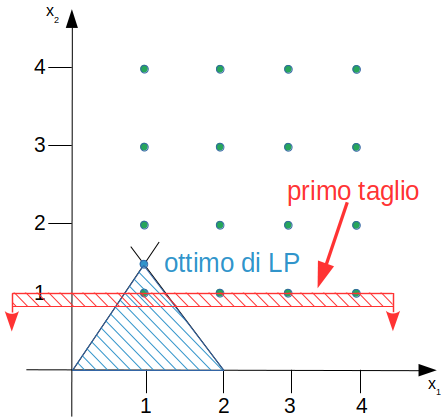
\includegraphics[height=8cm]{images/graph13.png}}

Aggiungendo il cut al tableau ottimo precedente:
\begin{table}[!h]
	\centering
	\begin{tabular}{cccccccc}
				&                         & $x_{1}$ & $x_{2}$  & $x_{3}$ & $x_{4}$ & $s_{1}$ &  RHS  \\ \cline{2-8}
		z		& \multicolumn{1}{|l|}{1} & 0       & 0        & -1/4    & -1/4    & 0 & \multicolumn{1}{|l|}{-3/2} \\ \cline{2-8}
		$x_{1}$ & \multicolumn{1}{|l|}{0} & 1       & 0        & 1/6     & -1/6    & 0 & \multicolumn{1}{|l|}{1} \\
		$x_{2}$ & \multicolumn{1}{|l|}{0} & 0       & 1        & 1/4     & 1/4     & 0 & \multicolumn{1}{|l|}{3/2} \\
		$s_{1}$ & \multicolumn{1}{|l|}{0} & 0       & 0        & \textbf{-1/4}     & -1/4   & 1  & \multicolumn{1}{|l|}{1} \\ \cline{2-8}
	\end{tabular}
\end{table}

Continuando con il simplesso duale:
\begin{table}[!h]
	\centering
	\begin{tabular}{cccccccc}
				&       				  & $x_{1}$ & $x_{2}$  & $x_{3}$ & $x_{4}$ & $s_{1}$ &  RHS  \\ \cline{2-8}
		z		& \multicolumn{1}{|l|}{1} & 0       & 0        & 0       & 0       & -1      & \multicolumn{1}{|l|}{-1} \\ \cline{2-8}
		$x_{1}$ & \multicolumn{1}{|l|}{0} & 1       & 0        & 0       & -1/3    & 2/3     & \multicolumn{1}{|l|}{2/3} \\
		$x_{2}$ & \multicolumn{1}{|l|}{0} & 0       & 1        & 0       & 0       & 1       & \multicolumn{1}{|l|}{1} \\
		$s_{1}$ & \multicolumn{1}{|l|}{0} & 0       & 0        & 1       & 1       & -4      & \multicolumn{1}{|l|}{2} \\ \cline{2-8}
	\end{tabular}
\end{table}

Dalla riga di $x_{1}$ si ha il cut:
\begin{equation*}
-\frac{2}{3}x_{4} - \frac{2}{3}s_{1} + s_{2} = - \frac{2}{3}
\end{equation*}

Il nuovo tableau, quindi, diviene:
\begin{table}[!h]
	\centering
	\begin{tabular}{ccccccccc}
				&       				  & $x_{1}$ & $x_{2}$  & $x_{3}$ & $x_{4}$ & $s_{1}$ & $s_{2}$ &  RHS  \\ \cline{2-9}
		z		& \multicolumn{1}{|l|}{1} & 0       & 0        & 0       & 0       & -1      & 0	   & \multicolumn{1}{|l|}{-1} \\ \cline{2-9}
		$x_{1}$ & \multicolumn{1}{|l|}{0} & 1       & 0        & 0       & -1/3    & 2/3     & 0       & \multicolumn{1}{|l|}{2/3} \\
		$x_{2}$ & \multicolumn{1}{|l|}{0} & 0       & 1        & 0       & 0       & 1       & 0       & \multicolumn{1}{|l|}{1} \\
		$s_{1}$ & \multicolumn{1}{|l|}{0} & 0       & 0        & 1       & 1       & -4      & 0       & \multicolumn{1}{|l|}{2} \\
		$s_{2}$ & \multicolumn{1}{|l|}{0} & 0       & 0        & 0       & -2/3    & -2/3    & 1       & \multicolumn{1}{|l|}{2/3} \\ \cline{2-9}
	\end{tabular}
\end{table}

e ottimizzando con li simplesso duale:
\begin{table}[!h]
	\centering
	\begin{tabular}{ccccccccc}
				&       				  & $x_{1}$ & $x_{2}$  & $x_{3}$ & $x_{4}$ & $s_{1}$ & $s_{2}$ &  RHS  \\ \cline{2-9}
		z		& \multicolumn{1}{|l|}{1} & 0       & 0        & 0       & 0       & -1      & -1/2	   & \multicolumn{1}{|l|}{-1} \\ \cline{2-9}
		$x_{1}$ & \multicolumn{1}{|l|}{0} & 1       & 0        & 0       & 0       & -1      & 0       & \multicolumn{1}{|l|}{1} \\
		$x_{2}$ & \multicolumn{1}{|l|}{0} & 0       & 1        & 0       & 0       & 1       & 0       & \multicolumn{1}{|l|}{1} \\
		$s_{1}$ & \multicolumn{1}{|l|}{0} & 0       & 0        & 1       & 0       & -5      & 3/2     & \multicolumn{1}{|l|}{2} \\
		$s_{2}$ & \multicolumn{1}{|l|}{0} & 0       & 0        & 0       & 1       & 1       & -3/2    & \multicolumn{1}{|l|}{1} \\ \cline{2-9}
	\end{tabular}
	\caption{Tableau ottimo.}
\end{table}

L'algoritmo converge in un numero finito di passi purché venga impiegata un'appropriata regola lessicografica per la scelta del pivot.

\subsubsection{Come evitare un numero indefinito di righe e colonne}
Qualora una variabile di slack $s_{i}$, associata all'$i$-esimo cut, entra in base, si elimina sia il cut sia la variabile $s_{i}$.

In questo modo il numero delle righe aggiunte (relative ai cuts) non supera $n-m$.

\section{Metodi Branch and Bound}
Sia $P_{0}$ un problema a cui corrisponde l'insieme $S_{0}$ di soluzioni ammissibili.

Ad esempio
\begin{displaymath}
P_{0}
\begin{cases}
\ Min\ \ cx\\
\ \ \ \ \ \ \ \ \ \ A x = b\\
\ \ \ \ \ \ \ \ \ \ x \ge 0\ e\:intero
\end{cases}
\end{displaymath}
\begin{equation*}
	S_{0}=\{x:Ax=b,\ x\ge 0\ intero\}
\end{equation*}

\subsection{Principio base dei metodi Branch and Bound}
Suddividere il problema $P_{0}$ nei sottoproblemi $P_{1},P_{2},\dots,P_{k}$ a cui corrispondono gli insiemi di soluzioni ammissibili $S_{1},S_{2},\dots,S_{k}$. La suddivisione è tale per cui:
\begin{equation*}
S_{1} \cup S_{2} \cup \dots \cup S_{k} = S_{0}
\end{equation*}
È evidente che:
\begin{equation*}
\min_{x \in S_{0}} cx = Min\{\min_{x\in S_{1}} cx, \min_{x\in S_{1}}cx,\dots,\min_{x\in S_{k}}cx\}
\end{equation*}
La risoluzione di ogni sottoproblema $P_{1},P_{2},\dots,P_{k}$ può risultare molto più semplice della risoluzione di $P_{0}$.\\
Possiamo rappresentare la suddivisione di $P_{0}$ in $P_{1},P_{2},\dots,P_{k}$ mediante un albero

\centerline{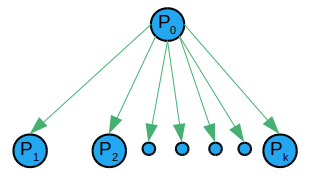
\includegraphics[height=4cm]{images/graph14.png}}

Nel caso in cui la riduzione di uno o più sottoproblemi risulti \emph{difficile} questi possono essere ulteriormente suddivisi.

Supponiamo che $P_{i}$ risulti difficile, allora può essere suddiviso nei sottoproblemi $P_{i1},P_{i2},\dots,P_{ik}$ a cui corrispondono gli insiemi di soluzioni ammissibili $S_{i1},S_{i2},\dots,S_{ik}$ tali che $S_{i1}\ \cup\ S_{i2}\ \cup\ \dots\ \cup\ S_{ik}\ =\ S_{i}$

\clearpage
Si ha il seguente albero

\centerline{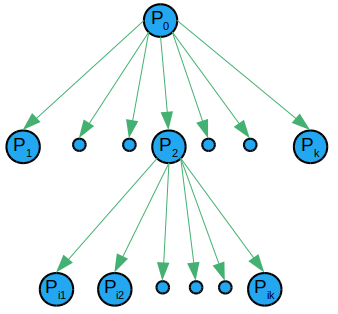
\includegraphics[height=5cm]{images/graph15.png}}

Risolvere $P_{0}$ equivale a risolvere $P_{1},\dots,P_{i-1},(P_{i1},P_{i2},\dots,P_{ir}),P_{i+1}\dots,P_{k}$.

Il processo di suddivisione di un problema in un numero finito di sottoproblemi viene chiamato \textbf{Branching}.\\
Una buona strategia di branching consiste nel suddividere $P_{i}$ nei sottoproblemi $P_{i1},P_{i2},\dots,P_{ir}$ in modo che, per ogni coppia $P_{i\alpha},P_{i\beta}$ con ($\alpha \neq \beta$), gli insiemi $S_{i\alpha}$ e $S_{i\beta}$ siano disgiunti.\\

\centerline{$S_{i\alpha} \cap S_{i\beta} = \emptyset$}

Se la condizione sopra è soddisfatta allora $\{S_{i},\dots,S_{ir}\}$ è una \textbf{partizione} di $S_{i}$.\\
Si noti che la condizione \textit{non è necessaria} ma rende computazionalmente efficiente il processo di branching.

\subsubsection{Esempi di Branching}
Si consideri il problema $P_{i}$ in $n$ variabili dove la variabile $x_{j}$ può assumere i valori $1$,$2$,$3$,$4$.
\centerline{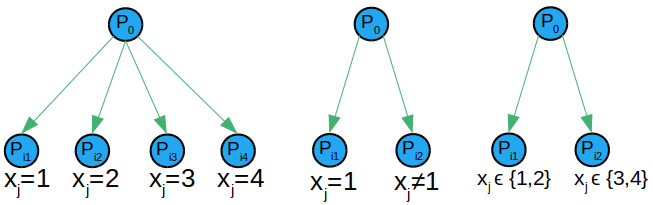
\includegraphics[height=4cm]{images/graph16.png}}
\clearpage

\subsection{Tipi di Branching}
Ogni sottoproblema che non può essere risolto può essere suddiviso in sottoproblemi più piccoli.\\
Dato un insieme di sottoproblemi da suddividere quale sottoproblema suddividere per primo?
\subsubsection{Depth-first search}
In 	questo tipo di branching il sottoproblema che viene suddiviso per primo è l'ultimo generato.\\
Ciò si ripete fino ad ottenere un sottoproblema che può essere risolto.\\

\centerline{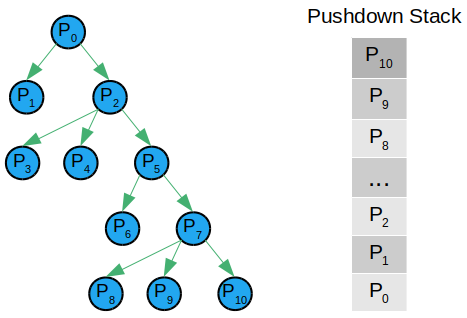
\includegraphics[height=8cm]{images/graph17.png}}

\textbf{Backtracing}: quando un sottoproblema è risolto viene scelto il penultimo sottoproblema generato e su questo viene effettuato il branching.

\subsubsection{Breadth-first search}
Il branching procede da livello a livello, ovvero il problema $P_{0}$ è suddiviso in $P_{1},P_{2},\dots,P_{k}$ che sono i sottoproblemi a livello 1.\\
Ogni sottoproblema a livello 1 viene suddiviso in un numero di sottoproblemi che costituiscono il livello 2.

In generale quando viene esaminato un sottoproblema a livello $K$ sono stati già esaminati tutti i sottoproblemi a livello $K-1$.
\clearpage
\begin{center}
	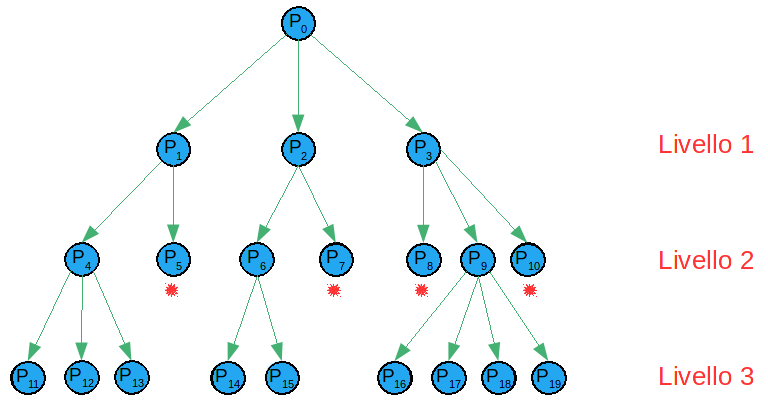
\includegraphics[height=8.2cm]{images/graph18.png}
	\captionof{figure}{* Problemi risolti}
\end{center}

\subsection{Bounds}
La ricerca della soluzione ottima di $P_{0}$ è completa quando sono stati risolti tutti i sottoproblemi generati.\\
Questo processo può essere migliorato calcolando, per ogni sottoproblema $P_{j}$ un \textbf{bound} (\textit{Lower Bound} se il problema è di minimizzazione).\\

\textbf{Lower Bound}: diremo che $LB_{i}$ è un lower bound al sottoproblema $P_{i}$ se
\begin{equation*}
LB_{i}\le\ \underset{x\in S_{i}}{Min}\{cx\}
\end{equation*}

\textbf{Upper Bound}: diremo che $UB_{i}$ è un upper bound al sottoproblema $P_{0}$ se
\begin{equation*}
UB_{i}\ge\ \underset{x\in S_{0}}{Min}\{cx\}
\end{equation*}
È possible trascurare il sottoproblema $P_{i}$ se $LB_{i}\ge UB$, infatti, poiché $LB_{i}\le \underset{x\in S_{i}}{Min}\{cx\}$ si avrebbe $\underset{x\in S_{i}}{Min}\{cx\}\ge UB$ e quindi il sottproblema $P_{i}$ non contiene la soluzione ottima.
\clearpage

\subsubsection{Calcolo del Lower Bound}
Sia dato il problema
\begin{displaymath}
P_{0}
\begin{cases}
\ Min\ \ z=cx\\
\ \ \ \ \ \ \ \ \ A x = b\\
\ \ \ \ \ \ \ \ \ x \ge 0\ e\:intero
\end{cases}
\end{displaymath}
Sia $z^{*}$ il costo della soluzione ottima di $P_{0}$.\\
I seguenti metodi producono validi lower bound a $P_{0}$.

\subsubsection{Rilassamento continuo}

Si ignori il vincolo $x$ intero; il problema risultante è risolvibile con la programmazione lineare.\\
Sia $z_{LP}^{*}$ il costo di tale soluzione; si ha
\begin{equation*}
	z_{LP}^{*}\le z^{*}
\end{equation*}
\begin{itemize}
	\item Se la soluzione del problema continuo è intera allora è anche la soluzione ottima intera e quindi $z_{LP}^{*}=z^{*}$;
	\item Se la soluzione è frazionaria allora può essere usato un metodo Branch \& Bound per trovare la soluzione ottima intera.
\end{itemize}

\textbf{Esempio.}

\centerline{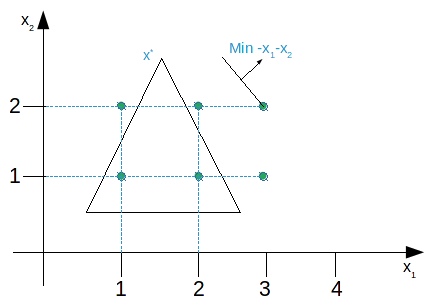
\includegraphics[height=6cm]{images/graph19.png}}
Rilassamento continuo $x^{*}=(\frac{3}{2},\frac{5}{2}),\ z_{LP}^{*}=cx^{*}=-4$

$P_{0}$ è suddiviso in due sottoproblemi $P_{1}\ e\ P_{2}$
\begin{itemize}
	\item $P_{1}$ imponiamo che $x_{1}\le 1$
	\item $P_{2}$ imponiamo che $x_{1}\ge 2$
\end{itemize}

\centerline{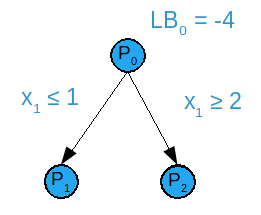
\includegraphics[height=4cm]{images/graph20.png}}
Si usi una strategia Depth-First e quindi si esamini il problema $P_{2}$.

\textbf{Esame del sottoproblema $\boldsymbol{P_{2}}$}

Il lower bound si ottiene imponendo il vincolo $x_{1}\ge 2$.

\centerline{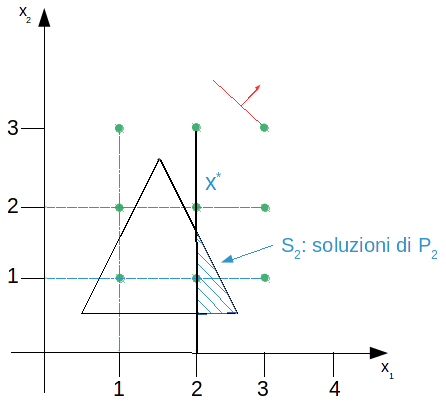
\includegraphics[height=6.5cm]{images/graph21.png}}
L'ottimo per $P_{2}$ è $z_{LP}^{*}=-3.5$ con componenti $x_{1}^{*}=2$ e $1<x_{2}^{*}<2$

Il problema $P_{2}$ viene suddiviso in $P_{3}$ e $P_{4}$ dove
\begin{itemize}
	\item $P_{3}$ imponiamo $x_{1}\ge 2$ e \underline{$\boldsymbol{x_{2}\le 1}$}
	\item $P_{4}$ imponiamo $x_{1}\ge 2$ e \underline{$\boldsymbol{x_{2}\ge 2}$}
\end{itemize}

\centerline{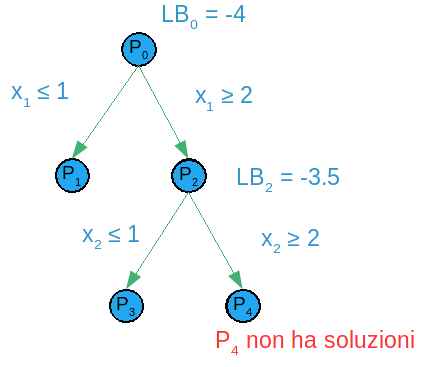
\includegraphics[height=6cm]{images/graph22.png}}

\textbf{Esame del sottoproblema $P_{3}$}

\centerline{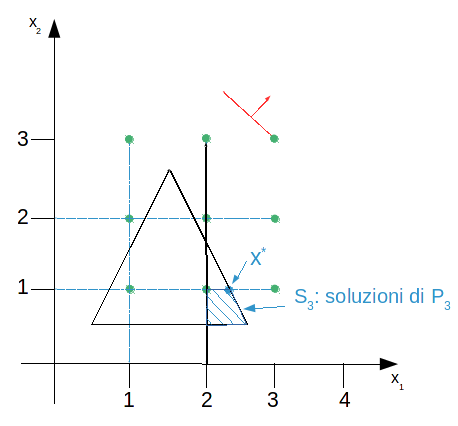
\includegraphics[height=9cm]{images/graph23.png}}

L'ottimo di $P_{3}$ è $z_{LP}^{*}=-3.25$ con componenti $x_{2}^{*}=1$ e $2 < x_{1}^{*} < 3$.

Il problema $P_{3}$ viene suddiviso in $P_{5}$ e $P_{6}$ dove
\begin{itemize}
	\item $P_{5}$ imponiamo $x_{1}\ge 2$, $x_{2}\le 1$ e \underline{$\boldsymbol{x_{1}\le 2}$}
	\item $P_{6}$ imponiamo $x_{1}\ge 2$, $x_{2}\le 2$ e \underline{$\boldsymbol{x_{1}\ge 3}$}
\end{itemize}

\centerline{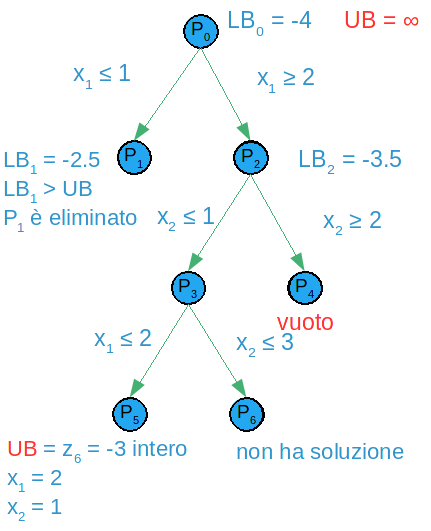
\includegraphics[height=9cm]{images/graph24.png}}

Al nodo dell'albero, corrispondente al problema $P_{5}$ si è ottenuta la prima soluzione ammissibile di $P_{0}$ di costo $-3$. Quindi poniamo \textbf{$UB = 3$}.\\
Il backtracking conduce ad esaminare il problema $P_{1}$

\centerline{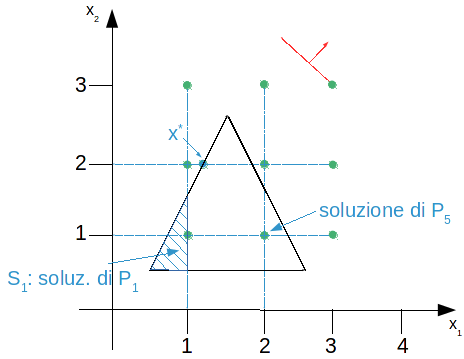
\includegraphics[height=7.5cm]{images/graph25.png}}

La soluzione ottima di $P_{1}$ è $z_{LP}^{*}=-2.5$, quindi, $LB_{1}=-2.5$ e poiché $LB_{1}>UB$ il sottoproblema $P_{1}$ non può condurre ad alcuna soluzione migliore di quella trovata per $P_{5}$.

Essendo stati esaminati tutti i nodi dell'albero l'algoritmo termina e $z^{*}=-3$ è la soluzione ottima.

\subsubsection{Eliminazione di alcuni vincoli}
Si consideri il problema
\begin{displaymath}
P_{0}
\begin{cases}
\ Min\ \ z=cx\\
\ \ \ \ \ \ \ \ \ \ A x = b\ \ m_{1}\ vincoli\\
\ \ \ \ \ \ \ \ \ \ Dx=h\ \ m_{2}\ vincoli\\
\ \ \ \ \ \ \ \ \ \ x\ge 0\ \ intero
\end{cases}
\end{displaymath}
Si consideri il problema RP che deriva da $P_{0}$ eliminando i vincoli $Ax=b$
\begin{displaymath}
RP
\begin{cases}
\ Min\ \ z_{RP}=cx\\
\ \ \ \ \ \ \ \ \ \ Dx=b\\
\ \ \ \ \ \ \ \ \ \ x \ge 0\ e\:intero
\end{cases}
\end{displaymath}
Sia $z_{RP}^{*}$ il valore ottimo di RP; si ha
\begin{equation*}
	z_{RP}^{*}\le z^{*} \ \ \ \ \ (z^{*}\textnormal{ ottimo di } P_{0})
\end{equation*}
L'estensione di questo metodo è il Rilassamento Lagrangiano mediante il quale è possibile tener conto dei vincoli rilassati nella funzione obiettivo.

\subsubsection{Rilassamento Surrogato}
Sia dato il problema
\begin{displaymath}
P_{0}
\begin{cases}
\ Min\ \ z=cx\\
\ \ \ \ \ \ \ \ \ \sum_{j=1}^{n}a_{ij}x_{j}\ge b_{i}\ \ i=1,\dots,m_{1}\\
\ \ \ \ \ \ \ \ \ Dx=h\ \ m_{2}\ vincoli\\
\ \ \ \ \ \ \ \ \ x\ge 0\ \ intero
\end{cases}
\end{displaymath}
Si consideri il problema che si ottiene da $P_{0}$ sostituendo i primi $m_{1}$ vincoli $a^{i}x\ge b_{i}$ con una loro combinazione lineare
\begin{displaymath}
SP
\begin{cases}
\ Min\ \ z_{SP}=cx\\
\ \ \ \ \ \ \ \ \ \sum_{j=1}^{m_{1}}\pi_{i}\sum_{j=1}^{n}a_{ij}^{j}x_{j}\ge \sum_{i=1}^{m_{1}}\pi_{i}b_{i}\ \ \pi_{i}\ge 0\\
\ \ \ \ \ \ \ \ \ Dx=h\ \ m_{2}\ vincoli\\
\ \ \ \ \ \ \ \ \ x\ge 0\ \ intero
\end{cases}
\end{displaymath}
$z_{SP}^{*}$, ottimo di SP, è un valido lower bound a $P_{0}$.

\subsection{Rilassamento lineare e surrogato}
\begin{displaymath}
P
\begin{cases}
\ z^{*}=\ Min\ cx\\
\ \ \ \ \ \ \ \ \ s.t.\ Ax\ge b\\
\ \ \ \ \ \ \ \ \ x\ge 0\ \ intero
\end{cases}
\end{displaymath}
Rilassamento lineare
\begin{displaymath}
LP
\begin{cases}
\ z_{LP}^{*}=\ Min\ cx\ \ \ \ \ \ \ =\ Max\ w b\\
\ \ \ \ \ \ \ \ \ \ \ s.t.\ Ax\ge b\ \ \ \ \ \ \ \ \ \ w A\le c\\
\ \ \ \ \ \ \ \ \ \ \ x\ge 0\ \ intero\ \ \ \ \ \ \ w \ge 0
\end{cases}
\end{displaymath}
Sia $w^{*}$ la soluzione duale ottima.
\begin{displaymath}
SP
\begin{cases}
\ z_{SP}^{*}=\ Min\ cx\\
\ \ \ \ \ \ \ \ \ \ \ (w^{*}A)x\ge w^{*}b\\
\ \ \ \ \ \ \ \ \ \ \ x\ge 0\ \ intero
\end{cases}
\end{displaymath}
Ottenuto tramite \textbf{rilassamento surrogato}.

\clearpage
\subsubsection{Teorema}

$z_{SP}^{*}\ge z_{LP}^{*}$\\
Poiché $w^{*}$ è la soluzione ottima del duale di LP si ha
\begin{equation*}
	z_{LP}^{*}=w^{*}b\ \ \ \textnormal{ e }\ \ \ c-w^{*}A\ge 0
\end{equation*}
Sia $x^{*}$ la soluzione ottima intera di SP; si ha:
\begin{equation}
	\label{eq:2.3}
	(c-w^{*}A)x^{*}\ge 0\ \ \ \textnormal{ ovvero }\ \ \ cx^{*}\ge w^{*}Ax^{*} 
\end{equation}
ma anche (da SP):
\begin{equation}
	\label{eq:2.4}
	w^{*}Ax^{*}\ge w^{*}b
\end{equation}
Da \ref{eq:2.3} e \ref{eq:2.4}:
\begin{equation*}
	cx^{*}\ge w^{*}Ax^{*}\ge w^{*}b=z^{*}_{LP}
\end{equation*}
ovvero
\begin{equation*}
	z^{*}_{SP}=cx^{*}\ge z_{LP}^{*}
\end{equation*}
$\square$

\section{Assegnamento Generalizzato}
Allocazione ottimale di $n$ oggetti in $m$ contenitori in modo che ogni oggetto sia assegnato ad un solo contenitore e non sia superata la portata di ogni contenitore.\\
Indichiamo con:
\begin{itemize}
	\item[] $b_{i}: \textnormal{ portata del contenitore }i,\ i=1,\dots,m$
	\item[] $a_{ij}: \textnormal{ spazio del contenitore $i$ occupato dall'oggetto $j$ (se $j$ viene assegnato a $i$)}$
	\item[] $c_{ij}: \textnormal{ costo per assegnare al contenitore $i$ l'oggetto $j$}$
	\item[] $x_{ij}$:
	\begin{itemize}
		\item[] $=1$ se l'oggetto viene assegnato al contenitore $i$
		\item[] $=0$ altrimenti
	\end{itemize}
\end{itemize}

\subsection{Formulazione matematica}
\begin{flalign}
	& Min\;\,\sum_{i=1}^{m}\sum_{j=1}^{n}c_{ij}x_{ij} \\
	& \ \ \ \ \ \ \ \ \sum_{i=1}^{m}x_{ij}=1,\ \ j=1,\dots,n \label{eq:2.6}\\
	& \ \ \ \ \ \ \ \ \sum_{j=1}^{n}a_{ij}x_{ij}le b_{i},\ \ i=1,\dots,m \label{eq:2.7} \\
	& \ \ \ \ \ \ \ \ x_{ij}\in \{0,1\},\ \forall i,j
\end{flalign}
Dove:
\begin{itemize}
	\item[\ref{eq:2.6}] ogni oggetto $j$ deve essere assegnato ad un solo contenitore
	\item[\ref{eq:2.7}] il "peso" complessivo assegnato ad ogni contenitore $i$ non deve superare la portata $b_{i}$
\end{itemize}

\subsection{Rilassamento lagrangiano}

\subsubsection{(a) Rispetto ai vincoli \ref{eq:2.6}}
\begin{flalign*}
	& L(u)=Min\ \sum_{i=1}^{m}\sum_{j=1}^{n}c_{ij}x_{ij}-\overbrace{\sum_{j=1}^{n}u_{j}(\sum_{i=1}^{m}x_{ij}-1)}^{-u(Ax-b)} =\\
	& L(u)=Min\ \sum_{i=1}^{m}(\sum_{j=1}^{n}(c_{ij} -u_{j})x_{ij})+\sum_{j=1}^{n}u_{j} \\
	& \ \ \ \ \ \ \ \ \ \ \ \ \ s.t.\sum_{j=1}^{n}a_{ij}x_{ij}\le b_{i},\ i=1,\dots,m \\
	& \ \ \ \ \ \ \ \ \ \ \ \ \ x_{ij}\in\{0,1\}
\end{flalign*}
L'ottimo $L(u)$ si ottiene risolvendo $m$ problemi di \textit{Knapsack} per il contenitore $i$ del tipo:
\begin{flalign*}
	& z_{i}=Min\ \sum_{j=1}^{n}(c_{ij}-u_{j})x_{ij} \\
	& \ \ \ \ \ \ \ \ \ \ \ \ \ \ \sum_{j=1}^{n}a_{ij}x_{ij}\le b_{i} \\
	& \ \ \ \ \ \ \ \ \ \ \ \ \ \ x_{ij}\in\{0,1\}
\end{flalign*}
Per cui $L(u)=\sum_{i=1}^{m}z_{i}\sum_{j=1}^{n}u_{j}$

\textbf{Esempio.}

$m=2$ contenitori; $n=4$ oggetti.

\centerline{$a_{ij}=\begin{bmatrix}5 & 7 & 4 & 2 \\ 3 & 1 & 6 & 4\end{bmatrix}$
$c_{ij}=\begin{bmatrix}3 & 3 & 4 & 9 \\ 2 & 6 & -9 & 3\end{bmatrix}$}
$b=(30,12)$

Poniamo $u^{0}=0$ e $z^{*}=3$ (soluzione euristica iniziale)
\begin{flalign*}
	& L(u^{0})=\ \underset{x}{Min}\sum_{i=1}^{m}(\sum_{j=1}^{n}(c_{ij}-u_{j}^{0})x_{ij}+\sum_{j=1}^{n}u_{j}^{0}) \\
	& L(u^{0})=\ \underset{x}{Min}\ 3x_{11}+3x_{12}+4x_{13}+9x_{14}+2x_{21}+6x_{22}-9x_{23}+3x_{24}+0 \\
	& 5x_{11}+7x_{12}+4x_{13}+2x_{14} \le 30 \\
	& 3x_{21}+x_{22}+6x_{23}+4x_{24} \le 12 \\
	& x_{11},\dots,x_{24}\in \{0,1\}
\end{flalign*}
Si decompone in due problemi: $L(u^{0})=z_{1}+z_{2}+0$

\begin{displaymath}
1^{0} problema
\begin{cases}
z_{1}=\ Min\ 3x_{11}+3x_{12}+4x_{13}+9x_{14}\\
\ \ \ \ \ \ \ \ 5x_{11}+7x_{12}+4x_{13}+2x_{14}\le 30\\
\end{cases}
\end{displaymath}
Soluzione ottima: $z_{1}=0;\ x_{11}^{0}=x_{12}^{0}=x_{13}^{0}=x_{14}^{0}=0$
\begin{displaymath}
2^{0} problema
\begin{cases}
z_{1}=\ Min\ 2x_{21}+6x_{22}-9x_{23}+3x_{24}\\
\ \ \ \ \ \ \ \ 3x_{21}+x_{22}+6x_{23}+4x_{24}\le 12\\
\end{cases}
\end{displaymath}
Soluzione ottima: $z_{2}=-9;\ x_{21}^{0}=x_{22}^{0}=0,\ x_{23}^{0}=1,\ x_{24}^{0}=0$

Quindi $L(u^{0})=z_{1}+z_{2}+0=0-9+0=-9$

La soluzione di $L(u^{0})$ non soddisfa i vincoli \ref{eq:2.6}; infatti:\\  $x=(x_{11},x_{12},x_{13},x_{14},x_{21},x_{22},x_{23},x_{24})$\\
$x^{0}=(\ 0,\ \ 0,\ \ \ 0,\ \ \ \ 0,\ \ \ \ 0,\ \ \ 0,\ \ \ 1,\ \ \ 0)$

\begin{displaymath}
Vincoli\ \ref{eq:2.6}
\begin{cases}
x_{11}\ \ \ \ \ \ \ \ \ \ \ \ \ \ \ \ \ \ \ \ +x_{21}\ \ \ \ \ \ \ \ \ \ \ \ \ \ \ \ \ \ \ \ \ \ \ \ \ \ \ \ \ =1\ \ (j=1)\\
\ \ \ \ \ x_{12}\ \ \ \ \ \ \ \ \ \ \ \ \ \ \ \ \ \ \ \ \ \ \ \ +x_{22}\ \ \ \ \ \ \ \ \ \ \ \ \ \ \ \ \ \ \ \ =1\ \ (j=2)\\
\ \ \ \ \ \ \ \ \ \ x_{13}\ \ \ \ \ \ \ \ \ \ \ \ \ \ \ \ \ \ \ \ \ \ \ \ \ \ \ \ +x_{23}\ \ \ \ \ \ \ \ \ \ \ =1\ \ (j=3)\\
\ \ \ \ \ \ \ \ \ \ \ \ \ \ x_{14}\ \ \ \ \ \ \ \ \ \ \ \ \ \ \ \ \ \ \ \ \ \ \ \ \ \ \ \ \ \ \ \ \ +x_{24}\ \ =1\ \ (j=4)\\
\end{cases}
\end{displaymath}
Si noti che la soluzione di $L(u^{0})$ viola i vincoli \ref{eq:2.6} per $j=1,2,4$ mentre soddisfa quello per $j=3$.

\textbf{Aggiornamento delle penalità \{u\}}
\begin{equation*}
	 u^{k}=u^{k-1}\alpha_{k}\frac{(z^{*}-L(u^{k-1}))}{||Ax^{k-1}-b||^{2}}\ .\ (Ax^{k-1}-b)
\end{equation*}
Poniamo $k=1$ ed $\alpha_{1}=2;$ si è già assunto $z^{*}=3$
\begin{flalign*}
	& u_{j}^{k}=u_{j}^{k-1}-2\cdot\frac{(+3 - (-9))}{\sum_{j=1}^{n}(\sum_{i=1}^{m}x_{ij}-1)^2}\cdot(\sum_{i=1}^{m}x_{ij}-1) \\
	& u_{1}^{1}=u_{1}^{0}-2\cdot\frac{12}{3}\cdot(-1)=0+8=8 \\
	& u_{2}^{1}=u_{2}^{0}-2\cdot 4\cdot(-1)=0+8=8 \\
	& u_{3}^{1}=u_{3}^{0}-2\cdot 4\cdot(0)=0+0=0 \\
	& u_{4}^{1}=u_{4}^{0}-2\cdot 4\cdot(-1)=0+8=8
\end{flalign*}
\clearpage
\textbf{Calcolo di $\boldsymbol{L(u{1})}$}
\begin{equation*}
	L(u^{1})=\ Min\ \sum_{i=1}^{m}(\sum_{j=1}^{n}(c_{ij}-u_{j}^{1})x_{ij})+\sum_{j=1}^{n}u_{j}^{1}
\end{equation*}
$c_{ij}=\begin{bmatrix}3 & 3 & 4 & 9 \\ 2 & 6 & -9 & 3\end{bmatrix}$\\
$u^{1}=(8,8,0,8)$

Come fatto in precedenza $L(u^{1})=z_{1}+z_{2}+24$ dove:
\begin{displaymath}
1^{0}\ problema
\begin{cases}
z_{1}=\ Min\ 5x_{11}-5x_{12}+4x_{13}+x{14}\\
\ \ \ \ \ \ \ \ 5x_{11}+7x_{12}+4x_{13}+2x_{14}\le 30\\
\ \ \ \ \ \ \ \ x_{11},\dots,x_{14}\in\{0,1\}
\end{cases}
\end{displaymath}
Soluzione ottima: $z_{1}=-10;\ x_{11}^{1}=x_{12}^{1}=1;\ x_{13}^{1}=x_{14}^{1}=0$
\begin{displaymath}
2^{0}\ problema
\begin{cases}
z_{2}=\ Min\ -6x_{21}-2x_{22}-9x_{23}-5x{24}\\
\ \ \ \ \ \ \ \ 3x_{21}+x_{22}+6x_{23}+4x_{24}\le 12\\
\ \ \ \ \ \ \ \ x_{21},\dots,x_{24}\in\{0,1\}
\end{cases}
\end{displaymath}
Soluzione ottima: $z_{2}=-17;\ x_{21}^{1}=x_{22}^{1}=x_{23}^{1}=1;\ x_{24}^{1}=0$.

Quindi $L(u^{1})=z_{1}+z_{2}+24=-10-17+24=-3$.\\
I vincoli \ref{eq:2.6} sono violati dalla soluzione $x_{1}$ di $L(u^{1})$.

$x^{1}=(\ 1,\ \ 1,\ \ \ 0,\ \ \ \ 0,\ \ \ \ 1,\ \ \ 1,\ \ \ 1,\ \ \ 0)$

I vincoli impongono:
\begin{displaymath}
\begin{cases}
x_{11}\ \ \ \ \ \ \ \ \ \ \ \ \ \ \ \ \ \ \ \ +x_{21}\ \ \ \ \ \ \ \ \ \ \ \ \ \ \ \ \ \ \ \ \ \ \ \ \ \ \ \ \ =1\\
\ \ \ \ \ x_{12}\ \ \ \ \ \ \ \ \ \ \ \ \ \ \ \ \ \ \ \ \ \ \ \ +x_{22}\ \ \ \ \ \ \ \ \ \ \ \ \ \ \ \ \ \ \ \ =1\\
\ \ \ \ \ \ \ \ \ \ x_{13}\ \ \ \ \ \ \ \ \ \ \ \ \ \ \ \ \ \ \ \ \ \ \ \ \ \ \ \ +x_{23}\ \ \ \ \ \ \ \ \ \ \ =1\\
\ \ \ \ \ \ \ \ \ \ \ \ \ \ x_{14}\ \ \ \ \ \ \ \ \ \ \ \ \ \ \ \ \ \ \ \ \ \ \ \ \ \ \ \ \ \ \ \ \ +x_{24}\ \ =1\\
\end{cases}
\end{displaymath}
\emph{Tutti i vincoli, eccetto il terzo, sono violati!}

\textbf{Aggiornamento delle penalità}
Poniamo $k=2$ e manteniamo $\alpha_{2}=2$ in quanto $L(u^{1})>L(u^{0})$
\begin{flalign}
& u_{j}^{k}=u_{j}^{k-1}-\alpha_{2}\cdot\frac{(z^{*} -L(u^{k-1}))}{\sum_{j=1}^{n}(\sum_{i=1}^{m}x_{ij}-1)^2}\cdot(\sum_{i=1}^{m}x_{ij}-1) \\
& u_{1}^{2}=u_{1}^{1}-2\cdot\frac{6}{3}\cdot(1)=8-4=4 \\
& u_{2}^{2}=u_{2}^{1}-2\cdot 2\cdot(1)=8-4=4 \\
& u_{3}^{2}=u_{3}^{1}-2\cdot 2\cdot(0)=0-0=0 \\
& u_{4}^{2}=u_{4}^{1}-2\cdot 2\cdot(-1)=8+4=12
\end{flalign}

\textbf{Calcolo di $\boldsymbol{L(u^{2})}$}
\begin{equation}
L(u^{2})=\ Min\ \sum_{i=1}^{m}(\sum_{j=1}^{n}(c_{ij}-u_{j}^{2})x_{ij})+\sum_{j=1}^{n}u_{2}^{1}
\end{equation}
\begin{equation}
	L(u^{2})=z_{1}+z_{2}+20
\end{equation}
dove $z_{1}$ e $z_{2}$ sono i valori ottimi dei problemi sequenti

$c_{ij}=\begin{bmatrix}3 & 3 & 4 & 9 \\ 2 & 6 & -9 & 3\end{bmatrix}$\\
$u^{2}=(4,4,0,12)$
\begin{displaymath}
1^{0}\ problema
\begin{cases}
z_{1}=\ Min\ -x_{11}-x_{12}+4x_{13}-3x_{14}\\
\ \ \ \ \ \ \ \ 5x_{11}+7x_{12}+4x_{13}+2x_{14}\le 30\\
\ \ \ \ \ \ \ \ x_{11},\dots,x_{14}\in\{0,1\}
\end{cases}
\end{displaymath}
Soluzione ottima: $z_{1}=-5;\ x_{11}^{2}=x_{12}^{2}=1,\ x_{13}^{2}=0,\ x_{14}^{2}=1$
\begin{displaymath}
2^{0}\ problema
\begin{cases}
z_{2}=\ Min\ -2x_{21}+2x_{22}-9x_{23}-9x_{24}\\
\ \ \ \ \ \ \ \ 3x_{21}+x_{22}+6x_{23}+4x_{24}\le 12\\
\ \ \ \ \ \ \ \ x_{21},\dots,x_{24}\in\{0,1\}
\end{cases}
\end{displaymath}
Soluzione ottima: $z_{2}=-18;\ x_{21}^{2}=x_{22}^{2}=0,\ x_{23}^{2}=x_{24}^{2}=1$

Quindi $L(u^{2})=z_{1}+z_{2}+24=-5-18+20=-3$

L'unico vincolo violato è $x_{14}+x_{24}=1$; per cui
\begin{equation}
	u_{j}^{3}=u_{j}^{2}-\alpha_{3}\cdot\frac{(z^{*} -L(u^{2}))}{\sum_{j=1}^{n}(\sum_{i=1}^{m}x_{ij}-1)^2}\cdot(\sum_{i=1}^{m}x_{ij}-1)
\end{equation}
poniamo $\alpha_{3}=\alpha_{2}/2=1$. Le nuove penalità sono:
\begin{flalign}
& u_{1}^{3}=u_{1}^{2}-6\cdot(0)=4 \\
& u_{2}^{3}=u_{2}^{2}-6\cdot(0)=4 \\
& u_{3}^{3}=u_{3}^{2}-6\cdot(0)=0 \\
& u_{4}^{3}=u_{4}^{2}-6\cdot(1)=6
\end{flalign}
\textbf{Calcolo di $\boldsymbol{L(u^{3})=z_{1}+z_{2}+14}$ dove}
\begin{displaymath}
1^{0} problema
\begin{cases}
z_{1}=\ Min\ -x_{11}-x_{12}+4x_{13}+3x_{14}\\
\ \ \ \ \ \ \ \ \ \ \ \ \ \ \ \ \ 5x_{11}+7x_{12}+4x_{13}+2x_{14}\le 30\\
\ \ \ \ \ \ \ \ \ \ \ \ \ \ \ \ \ x_{11},\dots,x_{14}\in\{0,1\}
\end{cases}
\end{displaymath}
Soluzione ottima: $z_{1}=-2;\ x_{11}^{3}=x_{12}^{3}=1,\ x_{13}^{3}=x_{14}^{3}=0$

\begin{displaymath}
2^{0} problema
\begin{cases}
z_{2}=\ Min\ -2x_{21}+2x_{22}-9x_{23}-3x_{24}\\
\ \ \ \ \ \ \ \ \ \ \ \ \ \ \ \ \ 3x_{21}+x_{22}+6x_{23}+4x_{24}\le 12\\
\ \ \ \ \ \ \ \ \ \ \ \ \ \ \ \ \ x_{21},\dots,x_{24}\in\{0,1\}
\end{cases}
\end{displaymath}
Soluzione ottima: $z_{2}=-12;\ x_{21}^{3}=x_{22}^{3}=0,\ x_{23}^{3}=x_{24}^{3}=1$

Quindi $L(u^{2})=-2-12+14=0$.

$\square$ Si noti che $x^{3}$ è ammissibile e quindi la soluzione è ottima.

\subsubsection{(b) Rispetto ai vincoli \ref{eq:2.7}}
\begin{flalign*}
& L(u)=Min\ \overbrace{\sum_{i=1}^{m}\sum_{j=1}^{n}c_{ij}x_{ij}-\sum_{i=1}^{m}\lambda_{i}(\sum_{j=1}^{n}a_{ij}x_{ij}-b_{i})}^{cx - \lambda(Ax-b)} =\\
& L(u)=Min\ \sum_{j=1}^{n}(\sum_{i=1}^{m}(c_{ij} -\lambda_{i}a_{ij})x_{ij})+\sum_{i=1}^{m}\lambda_{i}b_{i} \\
& \ \ \ \ \ \ \ \ \ \ \ \ \ \ \ \ \ \ \ \ \sum_{i=1}^{m}x_{ij}=1 \\
& \ \ \ \ \ \ \ \ \ \ \ \ \ \ \ \ \ \ \ \ x_{ij}\in\{0,1\}
\end{flalign*}
L'ottimo si ottiene ponendo, per ogni $j$
\begin{equation*}
	x_{i^{*}j}=1\ \ \ \textnormal{ per }\ \ \  c_{i^{*}j}-\lambda_{i^{*}j}a_{i^{*}j}=\underset{i}{Min}\{c_{ij}-\lambda_{i}a_{ij}\}
\end{equation*}
Ovvero, ogni oggetto $j$ viene assegnato al contenitore $i^{*}$ rispetto al quale $j$ ha costo minimo.

\textbf{Esempio} \textit{(Problema precedente con $m=2$, $n=4$)}

\centerline{$a_{ij}=\begin{bmatrix}5 & 7 & 4 & 2 \\ 3 & 1 & 6 & 4\end{bmatrix}$
	$c_{ij}=\begin{bmatrix}3 & 3 & 4 & 9 \\ 2 & 6 & -9 & 3\end{bmatrix}$}
$b=(30,12)$

Poniamo $\lambda=(0,0)$ e assumiamo $z^{*}=3$ (come in precedenza).
\begin{flalign*}
	& L(\lambda^{0})=Min\ \sum_{j=1}^{n}(\sum_{i}^{m}(c_{ij}-\lambda_{i}a_{ij})x_{ij}+\sum_{i=1}^{m}\lambda_{i}b_{i}) \\
	& L(\lambda^{0})=3x_{11}+3x_{12}+4x_{13}+9x_{14}+2x_{21}+6x_{22}-9x_{23}+3x_{24}+0 \\
	& \begin{cases}
	x_{11}\ \ \ \ \ \ \ \ \ \ \ \ \ \ \ \ \ \ \ \ +x_{21}\ \ \ \ \ \ \ \ \ \ \ \ \ \ \ \ \ \ \ \ \ \ \ \ \ \ \ \ \ =1\\
	\ \ \ \ \ x_{12}\ \ \ \ \ \ \ \ \ \ \ \ \ \ \ \ \ \ \ \ \ \ \ \ +x_{22}\ \ \ \ \ \ \ \ \ \ \ \ \ \ \ \ \ \ \ \ =1\\
	\ \ \ \ \ \ \ \ \ \ x_{13}\ \ \ \ \ \ \ \ \ \ \ \ \ \ \ \ \ \ \ \ \ \ \ \ \ \ \ \ +x_{23}\ \ \ \ \ \ \ \ \ \ \ =1\\
	\ \ \ \ \ \ \ \ \ \ \ \ \ \ x_{14}\ \ \ \ \ \ \ \ \ \ \ \ \ \ \ \ \ \ \ \ \ \ \ \ \ \ \ \ \ \ \ \ \ +x_{24}\ \ =1\\
	\end{cases}
\end{flalign*}

Poniamo $x_{i^{*}j}=1$ dove $c_{i{*}j}=\underset{i}{Min}\{c_{ij}\};\ \ \forall j$

Dal $1^{o}$ vincolo $x_{11}=0,\ x_{21}=1$\\
Dal $2^{o}$ vincolo $x_{12}=1,\ x_{22}=0$\\
Dal $3^{o}$ vincolo $x_{13}=0,\ x_{23}=1$\\
Dal $4^{o}$ vincolo $x_{14}=0,\ x_{24}=1$\\

Quindi $L(\lambda^{0})=-1$

Soluzione ottenuta per $L(u^{0})$\\
$x=(x_{11},x_{12},x_{13},x_{14},x_{21},x_{22},x_{23},x_{24})$\\
$x^{1}=(\ 0,\ \ 1,\ \ \ 0,\ \ \ \ 0,\ \ \ \ 1,\ \ \ 0,\ \ \ 1,\ \ \ 1)$\\\\
$5x_{11}+7x_{12}+4x_{13}+2x_{14}\le 30$ soddisfatto\\
$3x_{21}+x_{22}+6x_{23}+4x_{24}\le 12$ violato!

Ulteriori iterazioni possono migliorare il lower bound\dots

\subsection{Algoritmo Branch \& Bound}
\textbf{(Ad esempio)}

\centerline{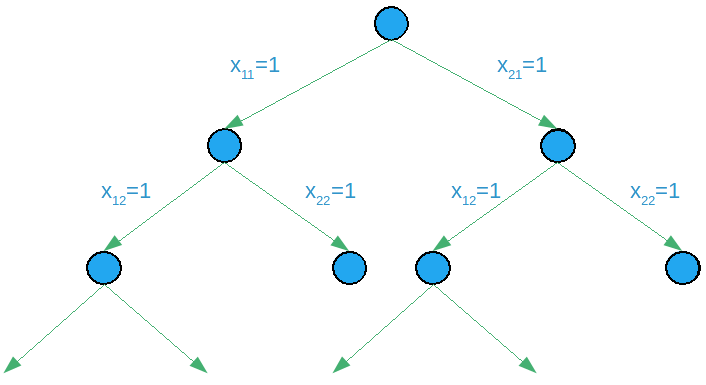
\includegraphics[height=8cm]{images/graph26.png}}
Ad ogni livello $j$ viene deciso in quale contenitore inserire l'oggetto $j$.

Da ogni nodo vengono generati $m$ nodi.